
\section{Introduction to Hybrid Place}
This chapter present one of the three theoretical approaches I have borrowed concepts to synthesise my framework in Chapter 6: A new way of designing for meaningfulness?. The theoretical background for Hybrid Place will often be referred to as it is, or simply Hybrid, as the thesis unfolds. This is a place-centred approach to the museum, and the four dimensions have both a formative application for the design of the data-gathering guides, as evident in the Appendix, along with the theoretical application into the framework in Chapter 6: A new way of designing for meaningfulness.


\section{Designing a hybrid place}
"Thanks to the development of ubiquitous and pervasive technologies, research focusing on the design of novel interactive artefacts has recently become more concerned with studying and understanding the spatial properties of the world" \autocite[p. 159]{hybridplace_ciolfi}. Bringing technologies beyond the desktop and into the world requires an ever-increasing interest in the \emph{physical environment} where interaction occurs \autocite[p. 159]{hybridplace_ciolfi}. Designing the interaction between ubiquitous technologies and users involves both a re-conceptualization of the interface as an assembly of tangible physical elements (including furniture and everyday objects), and importantly an understanding of the relationship between users and the physical space that is augmented by the technology \autocite[p. 159]{hybridplace_ciolfi}. Following the interest in the physical environment where interaction occurs, Ciolfi and Bannon discusses how geographical notions of space and place can aid designers in creating meaningful interactions between end-users and technologically augmented physical spaces. After reviewing literature that discusses the use of spatial concepts and metaphors within the interaction design field, they present a conceptual frame to design technologically enhanced environments for museums and exhibitions in particular. Their goal is to show how a place-centred approach can practically guide and support design, specifically within a setting that has seen many cases of technology introduction that have led to the visitors' distraction from the museum holdings, instead of extending and supporting the museum experience \autocite[p. 159-160]{hybridplace_ciolfi}.


% They have shown how new information technologies when used in museum environments, often suffer from a number of drawbacks; in particular, they argue that these technologies may hinder visitors appreciation of museum artefacts, their social interaction with others, and their appreciation of the place \autocite[p. 178]{hybridplace_ciolfi}.

Ciolfi and Bannon (2007) are particularly interested in the experience of place. They strive to understand the ways people come to ascribe meanings to particular places, and how certain places evoke complex webs of significance for people \autocite[p. 160]{hybridplace_ciolfi}. This is different from other similar research approaches that have attempted to use ideas from architecture and urban planning to inform the placement of interactive artefacts, e.g. \autocite{Cullen_book}, or noting how environment affects people's movement and interaction, e.g. \autocite{Alexander_book}. They base their articulation of place on the work of the geographer \autocite{Tuan_book}. According to Tuan, it is only natural that place is grounded in the physical, material reality of the world and that experience is shaped through physical sensing, exploration and habitation. On the basis of Tuan's conceptualisations, Ciolfi and Bannon propose an articulation of the concept of place that highlight the different dimensions as interconnected aspects of the individual experience:

\begin{figure}[H]
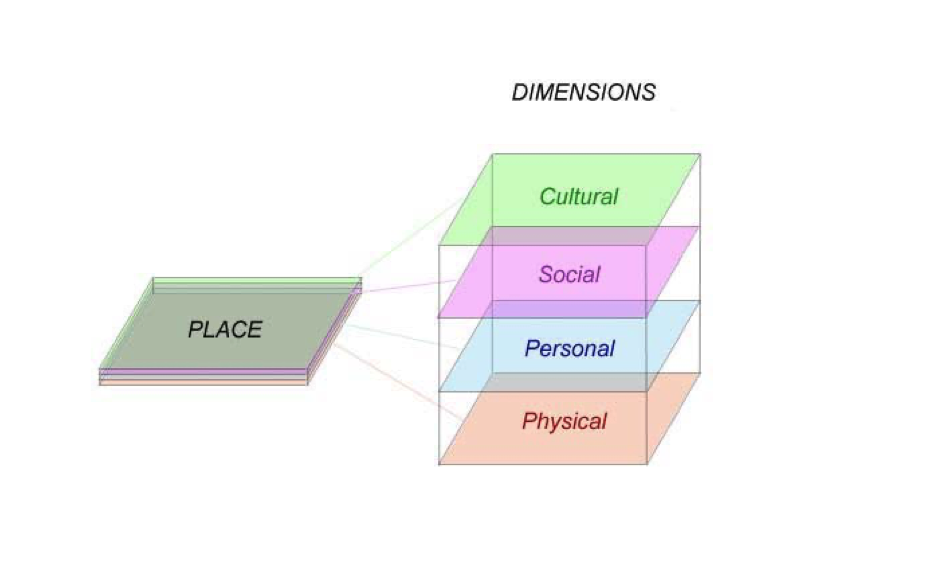
\includegraphics[width=12cm]{pictures/tuans_dimensions.png}
\caption{A representation of Tuans conceptualization of place}
\centering 
\autocite[p. 224]{spaceplace_ciolfi}
\end{figure}

The articulation of the four dimensions of place can help interaction design in interactive spaces by bringing aspects of individual traits and preferences, social interaction and cultural influences together with the physical features of the space \autocite[p. 163]{hybridplace_ciolfi}. These dimensions do not exist \emph{a priori}, but emerge and become visible in practise and experience as they lead to and emerge through peoples actions and activities in the museum space or with the installation \autocite[p. 163]{hybridplace_ciolfi}. As Ciolfi and Bannon explains it, each dimension is present at any moment of one's experience of place, but the experience itself is shaped by the dynamic interconnections among these dimensions. Each particular experience of the place is both individual and unique, although influenced by the presence of- and interaction with others. "Others" could be the other visitors in the museum, or e.g. a group of friends or family visiting together, as is expressed through the social dimension. In order to understand a place and its inhabitants, all four dimensions and their interplay with each other have to be taken into account \autocite[p. 162]{hybridplace_ciolfi}.

Ciolfi and Bannon argue that a place-centred approach can practically guide and support the design of museum experience. I have found this approach helpful when trying to understand how one can design interactive and meaningful museum experiences because it help position and argue for why and how the context e.g. surroundings and environmental qualities influences one's impression of the museum, the exhibition or a particular installation. I believe the concept of a hybrid place can help to understand interaction dynamics in the museum context. In addition to this, it provides a vocabulary and a theoretical lens to talk about and understand a specific experience with e.g. an interactive installation. The level of abstraction on the four dimensions provides an opportunity to incorporate different types of museum experiences. This can be useful in initial stages of a design process when you are getting to know a new museum context, providing a holistic lens to help read the room and learn its truth. 

% \par In my opinion, interactivity alone wont build a meaningful experience, it is a close "samspill" between the installations in the narrative path that the museum build, as well as a way to remember the place where you experienced something meaningful. I believe that over time, when perhaps months or years have passed and the details of the experience is forgotten, what remains is the memory of something meaningful happening in that place; the museum. That's what makes you want to come back to the space, or bring friends and family.


\section{Four dimensions}
When it comes to designing a hybrid place as researched by Ciolfi and Bannon (2007), the main contribution is the place-centred approach that provides the basis for a discussion of the place-related qualities in the museum of study. In Ciolfi and Bannon's case, they used the approach to highlight the limits of existing technologies and to propose the design of novel ones \autocite[p. 163]{hybridplace_ciolfi}, while in my case I am interested in using the place-centred approach to highlight meaningful relations in the museum.

Ciolfi and Bannon conducted a case study - the design of the interactive exhibition 'Re-Tracing the Past' at the Hunt Museum, Limerick - and the study shows how attention to place and its dimensions can inform design in quite concrete ways, and help in overcoming the problems of current interactive museum installations \autocite[p. 178]{hybridplace_ciolfi}. Through their development of their conceptualisation of 'place', involving people's lived experience of the physical space, based on \autocite{Tuan_book}'s work; they articulate four dimensions of place: physical, individual, social and cultural \autocite[p. 178]{hybridplace_ciolfi}. Their evaluations demonstrate that the exhibition they designed supported visitors engagement with museum artefacts, encouraged social interaction, discussion and debate, and allowed for personal and unique contributions to the place \autocite[p. 178]{hybridplace_ciolfi}.

\par
% This is what they did, and what I base my analysis/ lens on 
Through the case study of 'Re-tracing the Past', they derived four dimensions where their consideration of the multiple dimensions of peoples experience allowed to pinpoint issues to be dealt with in the design phase \autocite[p. 178]{hybridplace_ciolfi}.

\begin{itemize}
  \item \emph{The physical/structural dimension:} Relating to materials, structures and environmental factors. The exhibition should be aesthetically pleasing pleasing in order to merge harmonically with the museum; it should should be a space that favours participation and active discovery; it should be welcoming and friendly; it should support group interactions as well as individual's, and be accessible by different age groups.
  \item \emph{The personal dimension.} Related to the feeling and emotions we associate to a place, to the memories related to or evoked by it, to the personal knowledge and background we invest the place with while making sense of it. The exhibition should not have a prescribed sequence of actions in order to allow visitors to configure their visit; the exhibition should encourage visitors to express their opinions, comments and reflections and, to some extent, to leave their own trace; the visitors should feel welcomed and at ease. 
  \item \emph{The social dimension.} Related to social interaction and communication within the place, to the sharing of resources and memories, to social co-ordination and ethics, etc. Social interaction among groups of visitors should be supported and favoured. Also, the museum Docents should be encouraged to take part to the exhibition together with visitors.
  \item \emph{The cultural dimension.} Related to the rules, conventions and cultural identity of a place and of its inhabitants. The exhibition should be a representation of the museum's culture and identity. It should also suggest to visitors that - although located within a museum - the conventional cultural rules of behaviour in museums do not apply to it. People should feel free to interact actively with the installation, make themselves comfortable and so on.
\end{itemize}

I intend to use these four dimensions as a foundation for my scope in terms of data-gathering in the different museums and exhibitions that I’m visiting this semester. Ciolfi and Bannon explains how each dimension is present at any moment of one’s experience of a place, and the experience is shaped by the dynamic interconnections among these dimensions(p. 162), and after my museum visits I want to be able to analyse the museums and be enabled to identify some interconnections between the physical, personal, social and cultural dimension in a museum. I also intend to use the four dimensions in the synthesising of the framework of how to design meaningful interactive museum experiences.

\break
Their consideration of the multiple dimensions of people's experience allowed to pinpoint issues, four pitfalls or "problems" that arise:
\begin{itemize}
    \item How people appreciate the exhibit
    \item How people interact with eachother; and
    \item How people devise their own path through the exhibits and leave a trace of their presence in the space.
\end{itemize}

% \autocite[p. 168]{hybridplace_ciolfi}

\section{Introduction to Place as a dialogue}

This chapter presents a place-centred approach to the museum. The theoretical background from this chapter is used in the making of the framework presented in Chapter 6, and is often referred to as either Place as a dialogue or simply Place, as the thesis unfolds. 


\section{A dialogical approach to place}
John McCarthy and Luigina Ciolfi present what they call a dialogical approach to place, people, and technology. Dialogical is an adjective relating to or in the form of dialogue. I found this approach relevant in light of the climate debate, especially in terms of how the public discussion takes places both locally and globally at the same time because of social media. Could the "localness"  of the museum be one of its strengths in this type of discourse? 

 "Experience involves acting and being acted upon, sensing and feeling both, and transforming them into something emotionally and intellectually meaningful" \autocite[p. 250]{mccarthy_place}. 


 on how to solve climate- related issues, to the articles focus on the technological mediation of museum as a place in which people encounter and experience exhibited artefacts curated to fit the museums expository agency.

The sense people make of their experience—individual and collective—makes use of place and indeed makes or transforms place. As sensory and affective experience becomes transformed in thought and story, a museum (or anyother environment) can become a significant place for people and contributes in some meaningful way to transforming the people themselves \autocite[p. 250]{mccarthy_place}.

In Ciolfi and McCarthy’s opinion, frameworks that have been made to guide the design of interactive museum exhibitions developed in the field of museums studies, underplay aspects of visitor’s active sense making and interpretation. And that most practical and conceptual contributions from both museum studies and interaction design have fallen short of their potential to reflect on and design technologically mediated museum experiences partly because of the underdeveloped or under-articulated conceptualisations of visitor experience with which they work \autocite[p. 248]{mccarthy_place}



\section{Five dialogic principles}
The dialogical approach attends to the complexity and plurality of experience of place both as material and ideal, physical and cultural, sensory and reflective. Thus it suggests that analysis of experience of a place requires attention to both the immediate sensory transaction and the ways in which the immediate experience transforms in the telling \autocite[p. 251]{mccarthy_place}. They propose the following dimensions as building blocks of what they call a dialogical ontology that can prove to be useful in the design of and evaluation of interactive museum experiences:

From \autocite[]{}
\begin{itemize}
    \item \emph{Museum Experience is Relational.} Experience is seen in terms of the variety of relationships and practices of which it is constituted. One way to look at this variety is in terms of the relationships that sustain different museums, for example relationships between past and present, the building and the community, museum staff and visitors, exhibits and visitors. 
    
    \item \emph{Museum Experience is Open.} There is a sense in which the very idea of a digital artefact or installation in a museum plays on the boundary between two contrasting genres; fx digital and traditional. Beyond these and more genres, some museums play with the openness of experience by creating areas for enquiry, study, questioning and discussion, places that actively promote dialogue.

    \item \emph{Experiences in a Museum are at the Centre of a Variety of Sense-making Practises.} Environments, objects, artefacts and indeed exhibitions and museums attain meaning for people through their ongoing experience with and reflection on them. We interpret the situation in terms of our previous experiences and we reflect on our experience and our response to it. These processes give our experiences a narrative quality.
    
    \item \emph{Museum Experience Situates Artefacts in Narrative.} The narrative around them can be as important to experiencing them as the objects themselves. There is a sense in which we actually ‘make’ the experience by recounting it, as the expression of experience is both structured by and structures the experience. 
    
    \item \emph{Museum Experience is Sensitive to the Peculiarities of Space and Time.} Attending to the ways in which we make sense of experience introduces temporal and social dimensions to our account of experience. The temporal refers to the ways in which past and future are folded into the present experience as we make sense of it. Becoming present also changes past and future experience. We have seen how anticipating a future that includes explaining current experience to others changes current experience. Of course, it also transforms what future experience might be as we fill the future with those imagined explanations and encounters, which in time becomes the past transforming the present. 

\end{itemize}

I agree with and like where Ciolfi’s research is going, and have found Ciolfi and McCarthy’s dialogical dimensions useful as a supplement as to where I can include this as a perspective of the visitors museum experience, in the ongoing analysis of the four museum dimensions presented in section 3.2 designing hybrid places. I also find that these dialogical dimensions can prove useful when designing and conceptualize the interactive installations for this thesis. I believe these dialogical dimensions can give me the extended vocabulary to further explore and define specific concepts linked to the problem framings from section 1.1:

How can exhibition artefacts invite visitors to come together and discuss sustainability issues?\par
Can interactive installations encourage visitors to take more action in sustainability issues after the exhibition visit?\par
Can new/different interactions with natural objects contribute to increased climate consciousness and activism?\par


\section{Discursive qualities in a museum}
\par

To help look at what happens in a museum, Bal is guided by the notion that the gesture of showing can be considered a discursive act. According to her, exhibiting a subject through putting “things” on display, creates a subject/object dichotomy (Bal, p. 3). Dichotomy is a division or contrast between two things that are represented as being opposed or entirely different. The dichotomy enables the subject to make a statement about the object, while the object is there to prove evidence or the truth of the statement. The addressee for the statement is the visitor, viewer or reader (Bal, p. 3). The discourse surrounding the exposition, or, more precisely the discourse that is the exposition, is “constative”: informative and affirmative (Bal, p. 3). The very fact of exposing the object —presenting it while informing about it — impels the subject to connect the “present” of the object to the “past” of their making, functioning and meaning (Bal, p. 4). This is one of the levels giving the exposition a narrative quality. The other level where narrative can occur is the necessarily sequential nature of the visit, the “walking tour” (Bal, p.4). The “walking tour” bind the elements of the exposition for the viewer together, where the narrative of walking through a museum is comparable to the narrative of reading a book.

The reason for Bal’s attention to museums is the actual, concrete “literal” exhibition of things in museums and galleries. She proposes that the tools to conduct cultural analysis in museums, are best selected and employed as an integration of rhetoric and narratology. Rhetoric helps to “read” not just the artefacts in a museum, but also the museum and its exhibitions themselves (Bal, p. 7). While the narratological perspective provides meaning to the otherwise loose elements of such a reading (Bal, p. 7). Most importantly, the analysis aims to yield, one the one hand an integrated account of the discursive strategies put into effect by the museums expository agent (the curators), and, on the other hand, the effective process of meaning-making these strategies suggest to the visitor (Bal, p.7). The reading itself, then, becomes part of the meaning it yields.

(For my study of how one can design meaningful, interactive experiences in a museum space that addresses sustainability, this perspective is relevant because it enables me to look into the sustainability domain with the help of vocabulary derived from museology and cultural analysis. In similar museums, like heritage museums displaying ethnic types of discourses - cultural analysis has helped identify cultural moralism and imperialism in museums. I have a hypothesis that cultural analysis in museums addressing sustainability issues could reveal power structures or tensions in the museums dissemination and exhibitory practise. Or perhaps moralism?)

The book account for the museum itself being an expository agent and having an expository agency, and the exposition, both in the broader, general sense of “exposing an idea”, and in the specific sense of being an exhibition pointing at objects. By dissecting and putting forward the expository agent who is implicitly “speaking” throughout the exhibition design, about the objects on display, one can see how one comments on the other. The book also explains how different museums speak different “fictions” as they call it; where fx the Munch museum display art and is namely an art museum. Klimahuset display climate history and futuristic scenarios, and as I have read the book would classify it as an ethnographic museum. The genre to which a museum allegedly belongs to is in itself part of the frame that puts pressure on the meanings it will produce. The distinction between the ethnographic museum and the art museums can help us understand the importance of addressing this central discursivity and of interpreting its effects. The ethnographic museum conserves and exhibits artefacts, the art museum, works of art.

\section{Introduction to Sense-making}

This chapter presents research on sense-making in HCI, on how to support user’s active indexing in museums. Two conceptual notions is presented; spatio-contextual embedding and indexing, which together make Figure 5.1. 



. The theoretical background from this chapter is used in the making of the framework presented in Chapter 6, and is often referred to as either Place as a dialogue or simply Place, as the thesis unfolds. 

\section{What is an interactive meaningful experience?}

To be able to answer how one can design interactive meaningful experiences in a museum space that addresses sustainability, I will first have to explain what I mean when I talk about an interactive meaningful experience. In this section I will present research on sense-making in HCI, on how to support user’s active indexing in museums. This is the basis for understanding how visitors orient and understand, makes-sense-of, their surroundings and comprehend how fx. an installation is to be used. It can also in some way help us understand the relationship between attention span and engagement (as in sense-making being a pre-necessity to be able to meaning-making), how long time does the visitor spend in front of the installation before it gives up on it, because they cannot make sense of it. (bcz they dont understand it).

Eva Hornecker contributes to design/ hci knowledge on design for human agency, sense making, and mindful engagement with our environment. She present two conceptual notions; spatio-contextual embedding and indexing. These concepts serves and can be applied both in conceptual, analytical and in evaluating stages in the design process, and from the following article Hornecker presents 8 design strategies for the creation of spatio-contextual embedding and support of indexing. I intend to take with me these 8 design strategies in my synthesising of a framework to help design meaningful interactive museum experiences, where the strategies can be utilised in beginning or evaluative phases to aid in designing an interactive meaningful installation or experience.


\section{Meaning-making vs sense-making}
The two terms are similar, but in this thesis they have slightly different “functions” and is relevant in different “order”. The term sense-making is primarily used to describe and look at how someone makes sense of something. In a museum space - do they understand how something is to be used? When interacting with an interactive exhibition or installation, how intuitive is it to be used, and how long do people interact with it to “get it”. And is it clear why the installation is relevant in the museum space?

Meaning-making on the other hand is more than anything related to the reflective aspects of how something is made-sense of. It is more concerned with how the installation experience can give or take away reflections linked to the expository agency. As a designer one have to ask, or be able to answer, “what is it that this installation shall convey?” - and then look at how the interactive experience support that agency, in terms of the visitors reflections and after-thoughts somewhat align with it.

\section{The concept of Spatio-contextual embedding}


this is 100 direct quotation from article ::::::::: Based on case studies from a museum context, Hornecker present and illustrate the notion of “spatio-contextual embedding”, which conceptualises installation designs that augment real objects and environments while keeping primary focus on attention. Key for this “embeddedness” is that interaction is contextualised within a meaningful setting, creating relationships between system and environment. While retaining a focus on original objects or environments, it supports user’s active engagement and sense making by inviting, enticing, or forcing them to draw connections. At the heart of this is indexing. ::::::::::::: (Hornecker, p. 1)

The key takeaway is that design that is spatially contextualised and physically embedded, seem to engender and support indexing actions, and as a result of that increases the visitors engagement with its surroundings.


\section{The concept of Indexing}
There has been increased interest in the field of visitor studies and museum research in the details of visitor behaviour in museums, which is what the research done on indexing contributes to. (Hornecker, p. ??)

Hornecker’s working definition of indexing is explained as the mindful referencing back-and-forth between two representations or entities, comparing and relating them to each other and creating new meaning while doing so (Hornecker, p. 2). In the preface of the article we are presented to a story where a group of people are situated on a field trip to a hilltop, where the group make use of a panel with a simplified depiction of the view to make sense of and engage with the scenery. One of them point out a famous mountain on the panel, and then, points in the distance, saying its name, while the rest of them attempt to follow his reference. This is used as a simple example of what Hornecker refers to as the act of indexing.

Indexing practises support human sense-making and engages people with their surroundings (Hornecker, p. 39). Think of it as the mental process that happens when one tries to read the room, understand how something works, or how something is intended to be used. Indexing is the subtile interpretation act that manifests as sense-making. It is a useful concept for the interaction designer working in a museum or a similar exhibition domain, as a way to guide the design and evaluation of whether or not installations ‘makes sense’ for the visitor. It can be a helpful concept in terms of designing for the extension of time spent in front of/with the installation, and for rethinking the ‘unpopular’ installations, strengthening the exhibition experience as a whole.

Hornecker’s understanding of indexing is closer to the tradition of gesture studies and ethnography, which focus on the ways people coordinate their actions, in contrast to the semiotic tradition where the focus lies in the indexical sign’s ability to project or provide the visitor with the information needed to understand the context. Indexical expression are ubiquitous in our lives and an elementary part of our communication and coordination practises, as shown by conversation and ethnographic studies (Hornecker, p. 3). This linguistic-communicative understanding of indexing as suggested by Hornecker, is extended to include the notion of “indexing for yourself”, inspired by ideas which highlight how, for example, pointing can serve as a memory aid for individual cognition, using the external environment as a resource to aid cognition (Hornecker, p. 3). Which is why Hornecker’s notion of indexing is more positioned to expand the idea that people actively index to make connections between different things - that indexing is linked to the human action, not being a semiotic property of the artefact (Hornecker, p.5). Hornecker’s focus lies in identifying and understanding the user’s active indexing actions and in-detail investigation that takes place in the given situation, while investigating how technology explicitly can support and foster indexing (Hornecker, p. 2).


\section{Strategies for Creation of Spatio-Contextual Embedding and Support of Indexing}
A new issue emerging from the studies presented in Hornecker’s article is how to design for indexicality. This means more than just integrating systems into a context, it is about purposely enabling users to make comparisons and references in both directions (Hornecker, p. 34). The strategies are translated into a question format, as this can make conceptual work more accessible for designers who dislike the vocabulary of design rules and guidelines, preferring open phrasing(Hornecker, p. 34), and the focus is on what to achieve rather than to avoid (Hornecker, p. 34). All of the strategies go together to create “contextual embedding”, however considerations and trade-offs need to be considered when combining strategies that fits your project or domain. (Hornecker, p. 34).

I intend to use the strategies in conceptual stages of prototyping. As well for evaluation/ analysis of installations and museum visits I have conducted. And, like I said in the beginning of this chapter, I intend to take with me these 8 design strategies in the synthesising of the framework that can help design meaningful interactive museum experiences. 

Hornecker presents this table with eight strategies for the creation of spatio-contextual embedding and the support of indexing;

\begin{figure}[H]
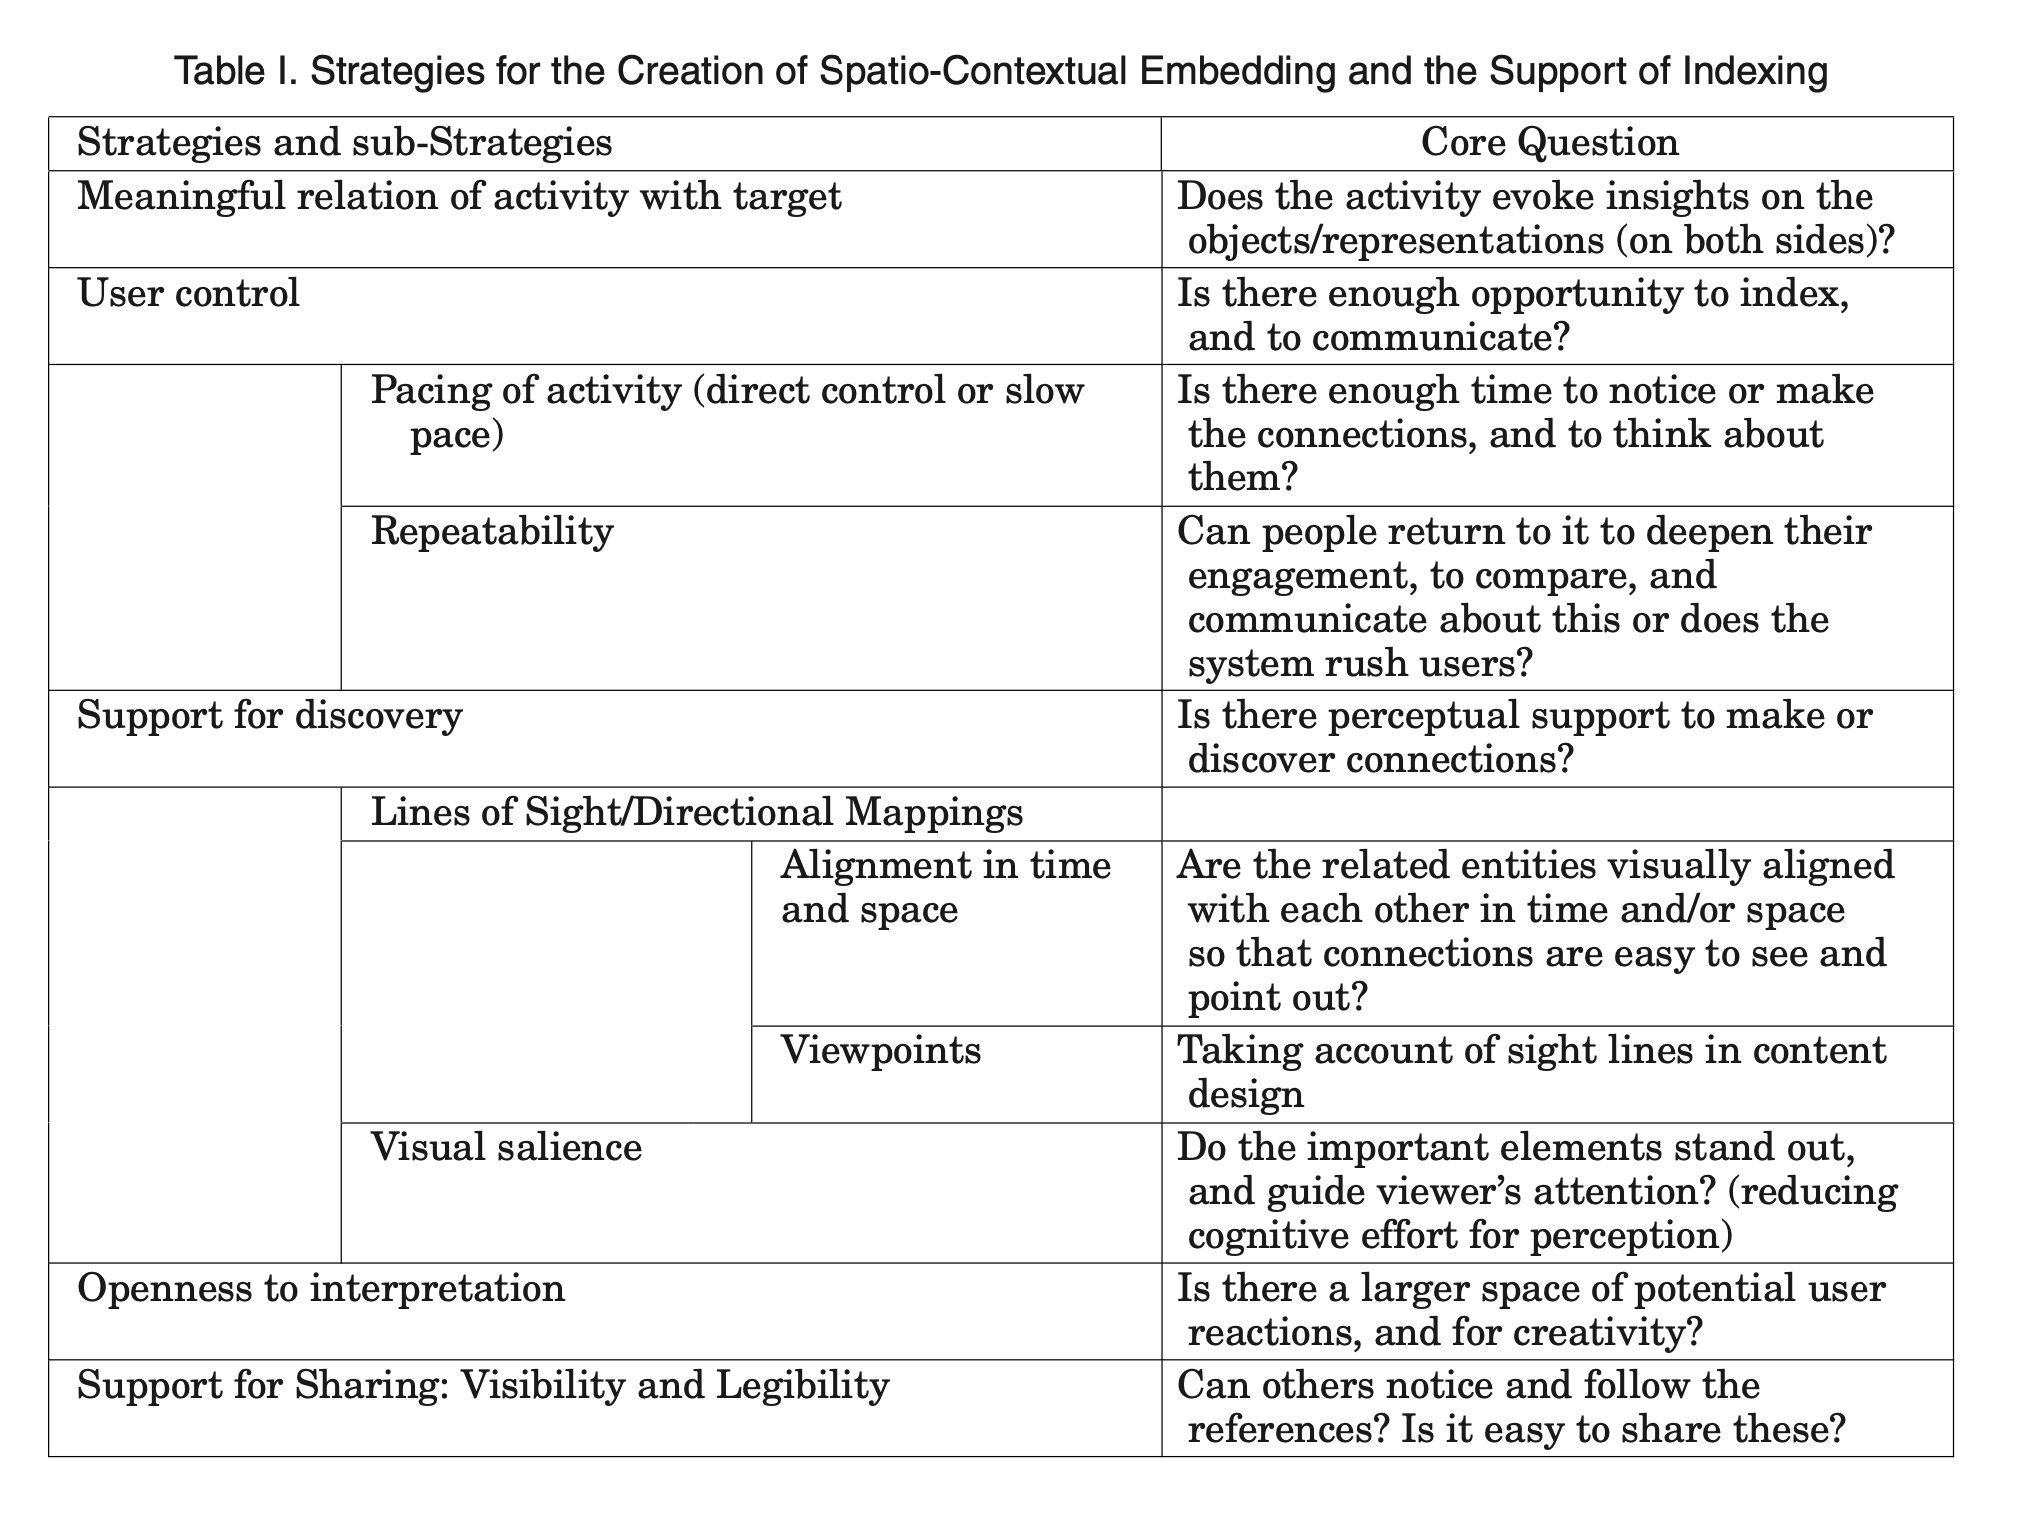
\includegraphics[width=12.5cm]{pictures/strategies.png}
\caption{Sense-making strategies}
\centering 
\end{figure}